\chapter{مدل سازی روش یادگیری ماشین}
در این بخش مدل سازی و پیاده سازی انجام طبقه بندی ترافیک با استفاده از یادگیری ماشین در پنج مرحله بررسی می‌شود. شکل زیر خلاصه ای از این مراحل را نشان می‌دهد.

\begin{figure}[!h]
\centerline{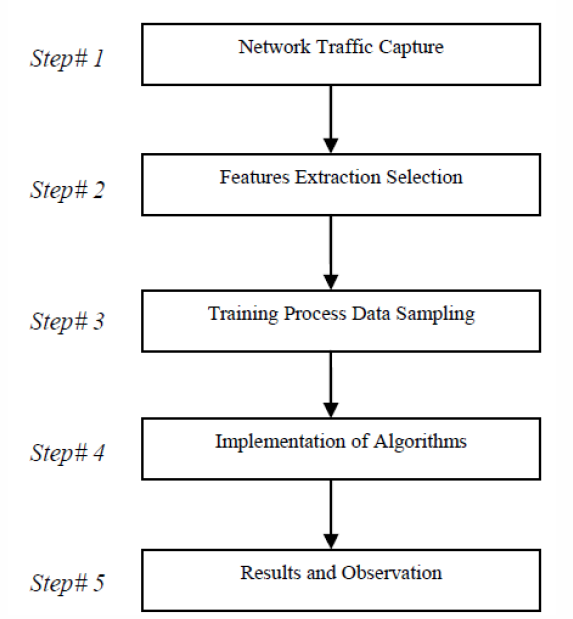
\includegraphics[width=0.6\textwidth]{steps.PNG}}
\caption[مدل پنج مرحله ای طبقه بندی ترافیک]{مدل پنج مرحله ای طبقه بندی ترافیک\cite{shafiq2016network}}
\end{figure}

همانطور که مشاهده می‌شود این پنج مرحله شامل جمع آوری داده، استخراج ویژگی ها، یادگیری نمونه، پیاده سازی الگوریتم و تحلیل نتایج می‌باشد، که در ادامه هر مرحله به اختصار توضیح داده می‌شود.

\section{جمع آوری داده}
اولین و مهم ترین بخش، جمع آوری داده یا به اصلاح گرفتن بسته\LTRfootnote{packet capture} های شبکه می باشد. ابزار های مختلفی برای این کار وجود دارد. از جمله معروف ترین ابزار ها در این زمینه وایرشارک\LTRfootnote{Wireshark} و تی سی پی دامپ\LTRfootnote{tcpdump} هستند که در پژوهش های مختلف از هر کدام از این ابزار ها استفاده شده است.

\section{استخراج ویژگی ها}
این مرحله که در پژوهش های مختلف غالبا با ابزارهای نت میت\LTRfootnote{Netmate} و پرل اسکریپت\LTRfootnote{Perl script} انجام می‌گیرد، ویژگی های خاصی از بسته ها استخراج می‌شود و با کمک آن ها دسته بند یادگیری ماشین\LTRfootnote{machine learning classifier} را آموزش می‌دهند. از جمله ویژگی های قابل استخراج می‌توان تعداد بسته ها، طول هر بسته، درگاه و پروتکل\LTRfootnote{protocol} مورد استفاده و غیره را نام برد. 

\section{یادگیری نمونه}
در مرحله ی سوم لازم است تا از داده های مورد نظر که در بخش اول بدست آمده، نمونه گیری انجام شود. از طرفی چون در این پژوهش از الگوریتم های یادگیری نظارت شده استفاده شده است، بر روی داده های دریافتی برچسب گذاری نیز انجام می‌شود تا بتوان به کمک آنها، بسته های ناشناخته را طبقه بندی کرد.

\section{پیاده سازی الگوریتم}
در این مرحله باید الگوریتم یادگیری ماشین مورد نظر بر روی داده های آموزش داده شده اعمال و پیاده سازی شوند. پژوهشگران معمولا به کمک ابزار وکا\LTRfootnote{Weka classification simulation tools}  این کار را انجام می‌دهند.


\section{بررسی و تحلیل نتایج}
در نهایت در بخش آخر ابراز وکا فرآیند تست روی داده ها را انجام می‌دهد و دقت ارزیابی انجام شده برای الگوریتم های مختلف را برای ما مشخص می‌کند.
با بررسی پژوهش های انجام شده بر روی شش الگوریتم یادگیری ماشین درخت تصمیم آر بی اف\LTRfootnote{RBF decision tree}، ماشین بردار پشتیبان\LTRfootnote{support vector machine (SVM)}، \lr{C4.5}، نزدیک ترین همسایه\LTRfootnote{nearest neighbor}، نیوبیز\LTRfootnote{naive bayes}، و شبکه بیز\LTRfootnote{bayesian network} نتایج زیر حاصل شده است. \cite{shafiq2016network, jamuna2013efficient}

\begin{table}[!h]
\caption{دقت طبقه بندی الگوریتم های مختلف یادگیری ماشین}
\centerline{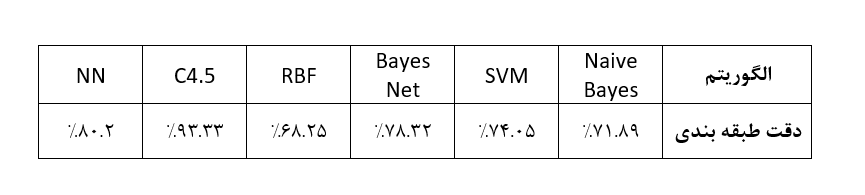
\includegraphics[width=1\textwidth]{accuracy.PNG}}
\end{table}

همانطور که در جدول نشان داده شده است، از بین الگوریتم های مورد استفاده در این پژوهش، با استفاده از الگوریتم یادگیری ماشین \lr{C4.5} توانسته ایم به دقت بیش از 93 درصد برای طبقه بندی ترافیک شبکه دست پیدا کنیم. الگوریتم نزدیک ترین همسایه نیز دقت تقریبا 80 درصدی را نشان می‌دهد. پس از آن برای الگوریتم های شبکه بیز، ماشین بردار پشتیبان و نیو بیز نیز دقتی بین 70 تا 80 درصد بدست آمده است.


\section{خلاصه}

در این بخش قدم به قدم با مراحل مدل سازی و پیاده سازی روش یادگیری ماشین آشنا شدیم و مشاهده کردیم که الگوریتم یادگیری ماشین \lr{C4.5} با دقتی معادل 5.93 درصد، بسته های شبکه را به درستی طبقه بندی می‌کند.